\chapter{Conclusion}
\label{chapter:6-CONCLUSION}
	
	%%%%%--------------------------------------------------------------------
	%%%%% OCCUPYING THE NICHE: Proposition d'une méthode d'annotation autour d'un \textit{Clustering Interactif}.
	%%%%%--------------------------------------------------------------------
	\section*{Proposition d'une nouvelle méthode d'annotation autour d'un \textit{Clustering Interactif}}
	\addcontentsline{toc}{section}{
		\protect\numberline{}
		Proposition d'une nouvelle méthode d'annotation autour d'un \textit{Clustering Interactif}
	}
	
		%%% Introduction, Revue de littérature et Rappel de la problématique (voir \textsc{Chapitre~\ref{chapter:2-REVUE-DE-LITTERATURE}}).
		Dans cette thèse, nous nous sommes intéressé à la tâche d'annotation, nécessaire à l'entraînement d'assistants conversationnels, et impliquant habituellement des experts du domaine à modéliser.
		Lors de notre revue de littérature, nous avons pu constater que l'annotation avait la réputation d'être une tâche complexe et subjective.
		Cette complexité provient notamment du besoin d'avoir des données représentatives du phénomène à reproduire, exerçant par conséquent une forte pression quant à la qualité de la base d'apprentissage à construire.
		Un projet d'annotation s'organise alors traditionnellement autour du cycle \texttt{MATTER}, une méthodologie durant laquelle la modélisation des textes en intentions est révisée plusieurs fois pour mieux s'adapter aux données du projet.
		Cependant, une telle organisation se révèle généralement coûteuse, entre autres à cause des nombreux ateliers de modélisation en mode essai-erreur, de la difficulté à manipuler des concepts abstraits (\textit{intentions}, \textit{entités}, ...), et du besoin de former les experts aux tâches d'analyse.
		Sur la base de ces constats, nous avons cherché une méthodologie d'annotation alternative en nous posant la question suivante : \textguillemets{\textbf{Comment assister la phase de modélisation de textes en intentions pour concevoir la base d'apprentissage d'un assistant conversationnel en impliquant des experts métiers pour leurs vraies compétences et en leur demandant un minimum de bagages analytiques ou techniques ?}}
		
		%%% Rappel proposition \texttt{Clustering Interactif} (voir \textsc{Chapitre~\ref{chapter:3-CLUSTERING-INTERACTIF}}).
		En choisissant de mettre l'accent sur les connaissances réelles des experts, nous avons proposé une approche de modélisation des textes en intentions utilisant un \texttt{Clustering Interactif}.
		Cette méthodologie repose sur la coopération entre l'Homme et la Machine :
		\begin{itemize}
			\item d'une part, la machine réalise un \textit{clustering} pour proposer une base initiale d'apprentissage ;
			\item d'autre part, l'expert métier annote des contraintes binaires entre les données dans le but d'affiner itérativement la base d'apprentissage proposée.
		\end{itemize}
		Une telle approche a l'avantage d'être plus instinctive, car les experts peuvent associer ou différencier les données en fonction de la similarité de leur cas d'usage, permettant ainsi de traiter les données comme ils le feraient professionnellement au quotidien.
		De plus, cette méthodologie définit clairement les rôles entre les parties : l'expert métier intervient uniquement pour transmettre ses connaissances métiers, et la machine se charge d'appliquer cette connaissance pour concevoir une modélisation stable et pertinente des textes en intentions.
		
		
		%%% Rappel études sur le \texttt{Clustering Interactif} (voir \textsc{Chapitre~\ref{chapter:4-ETUDES}}).
		Pour éprouver notre méthodologie d'annotation, nous avons réalisé un ensemble d'études réparties en six hypothèses : efficacité, efficience, coûts, pertinence, rentabilité et robustesse.
		Grâce à ces études, nous avons pu démontrer que notre méthode diminuait sensiblement la complexité de conception d'une base d'apprentissage, réduisant notamment la nécessité de formation des experts intervenant dans un projet d'annotation.
		Nous mettons à disposition une implémentation technique de cette méthode (algorithmes et interface graphique associée), ainsi qu'une étude des paramètres optimaux pour obtenir une base d'apprentissage cohérente en un minimum d'annotations (hypothèse d'efficacité et d'efficience).
		Nous réalisons également une étude de coûts (techniques et humains) permettant de confirmer que l'utilisation d'une telle méthode est réaliste dans un cadre industriel.
		Les trois dernières hypothèses (pertinence, rentabilité et robustesse) permettent de vérifier le comportement et les limites de notre technique, ouvrant ainsi la discussion sur les fonctionnalités et mécanismes de suivi nécessaires à sa mise en oeuvre.
		
		%%% Rappel guide sur le \texttt{Clustering Interactif} (voir \textsc{Chapitre~\ref{chapter:5-GUIDE}}).
		Nous dressons ensuite le bilan de notre méthodologie d'annotation sous la forme d'un guide d'utilisation synthétique.
		Afin que la méthode atteigne son plein potentiel, nous y fournissons un ensemble de conseils, notamment : (1) des recommandations visant à cadrer la stratégie d'annotation, (2) une aide à l'identification et à la résolution des divergences d'opinion entre annotateurs, (3) des indicateurs de rentabilité pour chaque intervention de l'expert, et (4) des méthodes d'analyse de la pertinence de la base d'apprentissage en cours de construction.
		
		%%% Conclusion finale.
		En conclusion, notre méthodologie d'annotation représente une réelle alternative aux stratégies d'annotation traditionnelles, permettant de valoriser les annotateurs pour les compétences qu'ils possèdent, et non pour les compétences dont le projet d'annotation a besoin.
		
		
	%%%%%--------------------------------------------------------------------
	%%%%% NICHE: Perspectives d'utilisation de notre \textit{Clustering Interactif}.
	%%%%%--------------------------------------------------------------------
	\section*{Perspectives d'utilisation de notre \textit{Clustering Interactif}}
	\addcontentsline{toc}{section}{
		\protect\numberline{}
		Perspectives d'utilisation de notre \textit{Clustering Interactif}
	}
		
		%%% Amélioration signification de l'implication des experts métiers.
		Nous avons pu montrer que cette thèse offrait une approche innovante pour concevoir une base d'apprentissage d'un assistant conversationnel, permettant d'impliquer les experts du domaine métier pour leurs vraies connaissances, tout en leur demandant un minimum de compétences analytiques et techniques.
		En effet, ces travaux prouvent qu'il est possible de contourner habilement la complexité d'une tâche d'annotation en reformulant judicieusement le problème exposé à l'annotateur, ouvrant ainsi la voie à des méthodes plus accessibles pour construire ces assistants.

		%%% Certes moins pour la gestion de dialogues (cf \textit{chatbot} génératif), mais probablement pour leur contrôle ; Application possible à des domaines autre que le texte (image, voix, données tabulaires, ...) si la modélisation est complexe
		Néanmoins, depuis $2023$, la conception de \textit{chatbot} s'est davantage tournée vers les approches génératives, celles-ci n'ayant plus besoin d'intentions pour gérer le dialogue.
		Mais malgré leurs performances encourageantes, ces approches manquent encore clairement de fiabilité, notamment en ce qui concerne les dérives de comportements et les risques d'hallucination ; de plus, une étape de modélisation reste nécessaire pour paramétrer certaines de leurs actions spécifiques (\textit{allumer la lumière, lancer un appel téléphonique, faire un virement bancaire, ...}).
		De ce fait, nous pensons que notre méthode d'annotation reste pertinente pour entraîner des assistants orientés par tâches, pour modéliser des mécanismes de contrôle, ou encore pour assister la conception de certains assistants hybrides.
		D'autres part, cette méthode pourrait facilement être adaptée à d'autres usages tout en conservant l'esprit d'une tâche d'annotation à choix binaires, permettant ainsi de rester au plus proche de la connaissance métier des opérateurs.
		
		%%% Ouverture vers Chatbot arena.
		\begin{leftBarAuthorOpinion}
			% Description générale de Chatbot arena.
			Parmi les techniques d'annotation récentes autour des modèles de génération de textes, nous sommes particulièrement attentifs à la méthode \textguillemets{\texttt{Chatbot Arena}} proposée par \texttt{LMSYS Org} (\cite{chiang-etal:2024:chatbot-arena-open}, voir \url{https://huggingface.co/spaces/lmsys/chatbot-arena-leaderboard} et \textsc{Figure~\ref{figure:6.2-PERSPECTIVES-CHATBOT-ARENA}}).
			Cette méthode consiste à comparer les réponses générées par deux modèles différents pour une même question en demandant à l'opérateur de choisir sa réponse préférée : soit la réponse de gauche est la meilleure (\textit{option \textguillemets{\texttt{{\faHandPointLeft}~A is better}}}), soit la réponse de droite est la meilleure (\textit{option \textguillemets{\texttt{{\faHandPointRight}~B is better}}}).
			Il est aussi possible de préciser si les deux réponses sont bonnes (\textit{option \textguillemets{\texttt{{\faHandshake}~Tie}}}) ou si aucune ne l'est (\textit{option \textguillemets{\texttt{{\faThumbsDown}~Both are bad}}}).
			Sur la base de ces annotations comparatives, un classement des modèles peut ensuite être établi en calculant leur score \texttt{elo}.
			
			% Parallèle entre Chatbot arena et Interactive Clustering.
			Nous avons constaté que notre \texttt{Clustering Interactif} et ce \texttt{Chatbot Arena} partagent plusieurs similitudes, bien que leurs objectifs soient différents (\textit{la modélisation en thématiques pour le premier, le classement de modèles génératifs pour le second}).
			Ces similitudes incluent un accent mis sur l'annotation binaire (\textit{{\faEquals}/{\faNotEqual} vs {\faHandPointLeft}/{\faHandPointRight}}) et sur la simplification de la tâche pour s'adapter aux compétences et aux connaissances des annotateurs.
			Ces points communs nous encouragent à croire qu'il sera possible d'adapter notre méthode d'annotation itérative basée sur un \texttt{Clustering Interactif} pour contribuer aux efforts de contrôle et d'alignement des modèles génératifs à venir.
		
			% Figure.
			\begin{figure}[H]
				\centering
				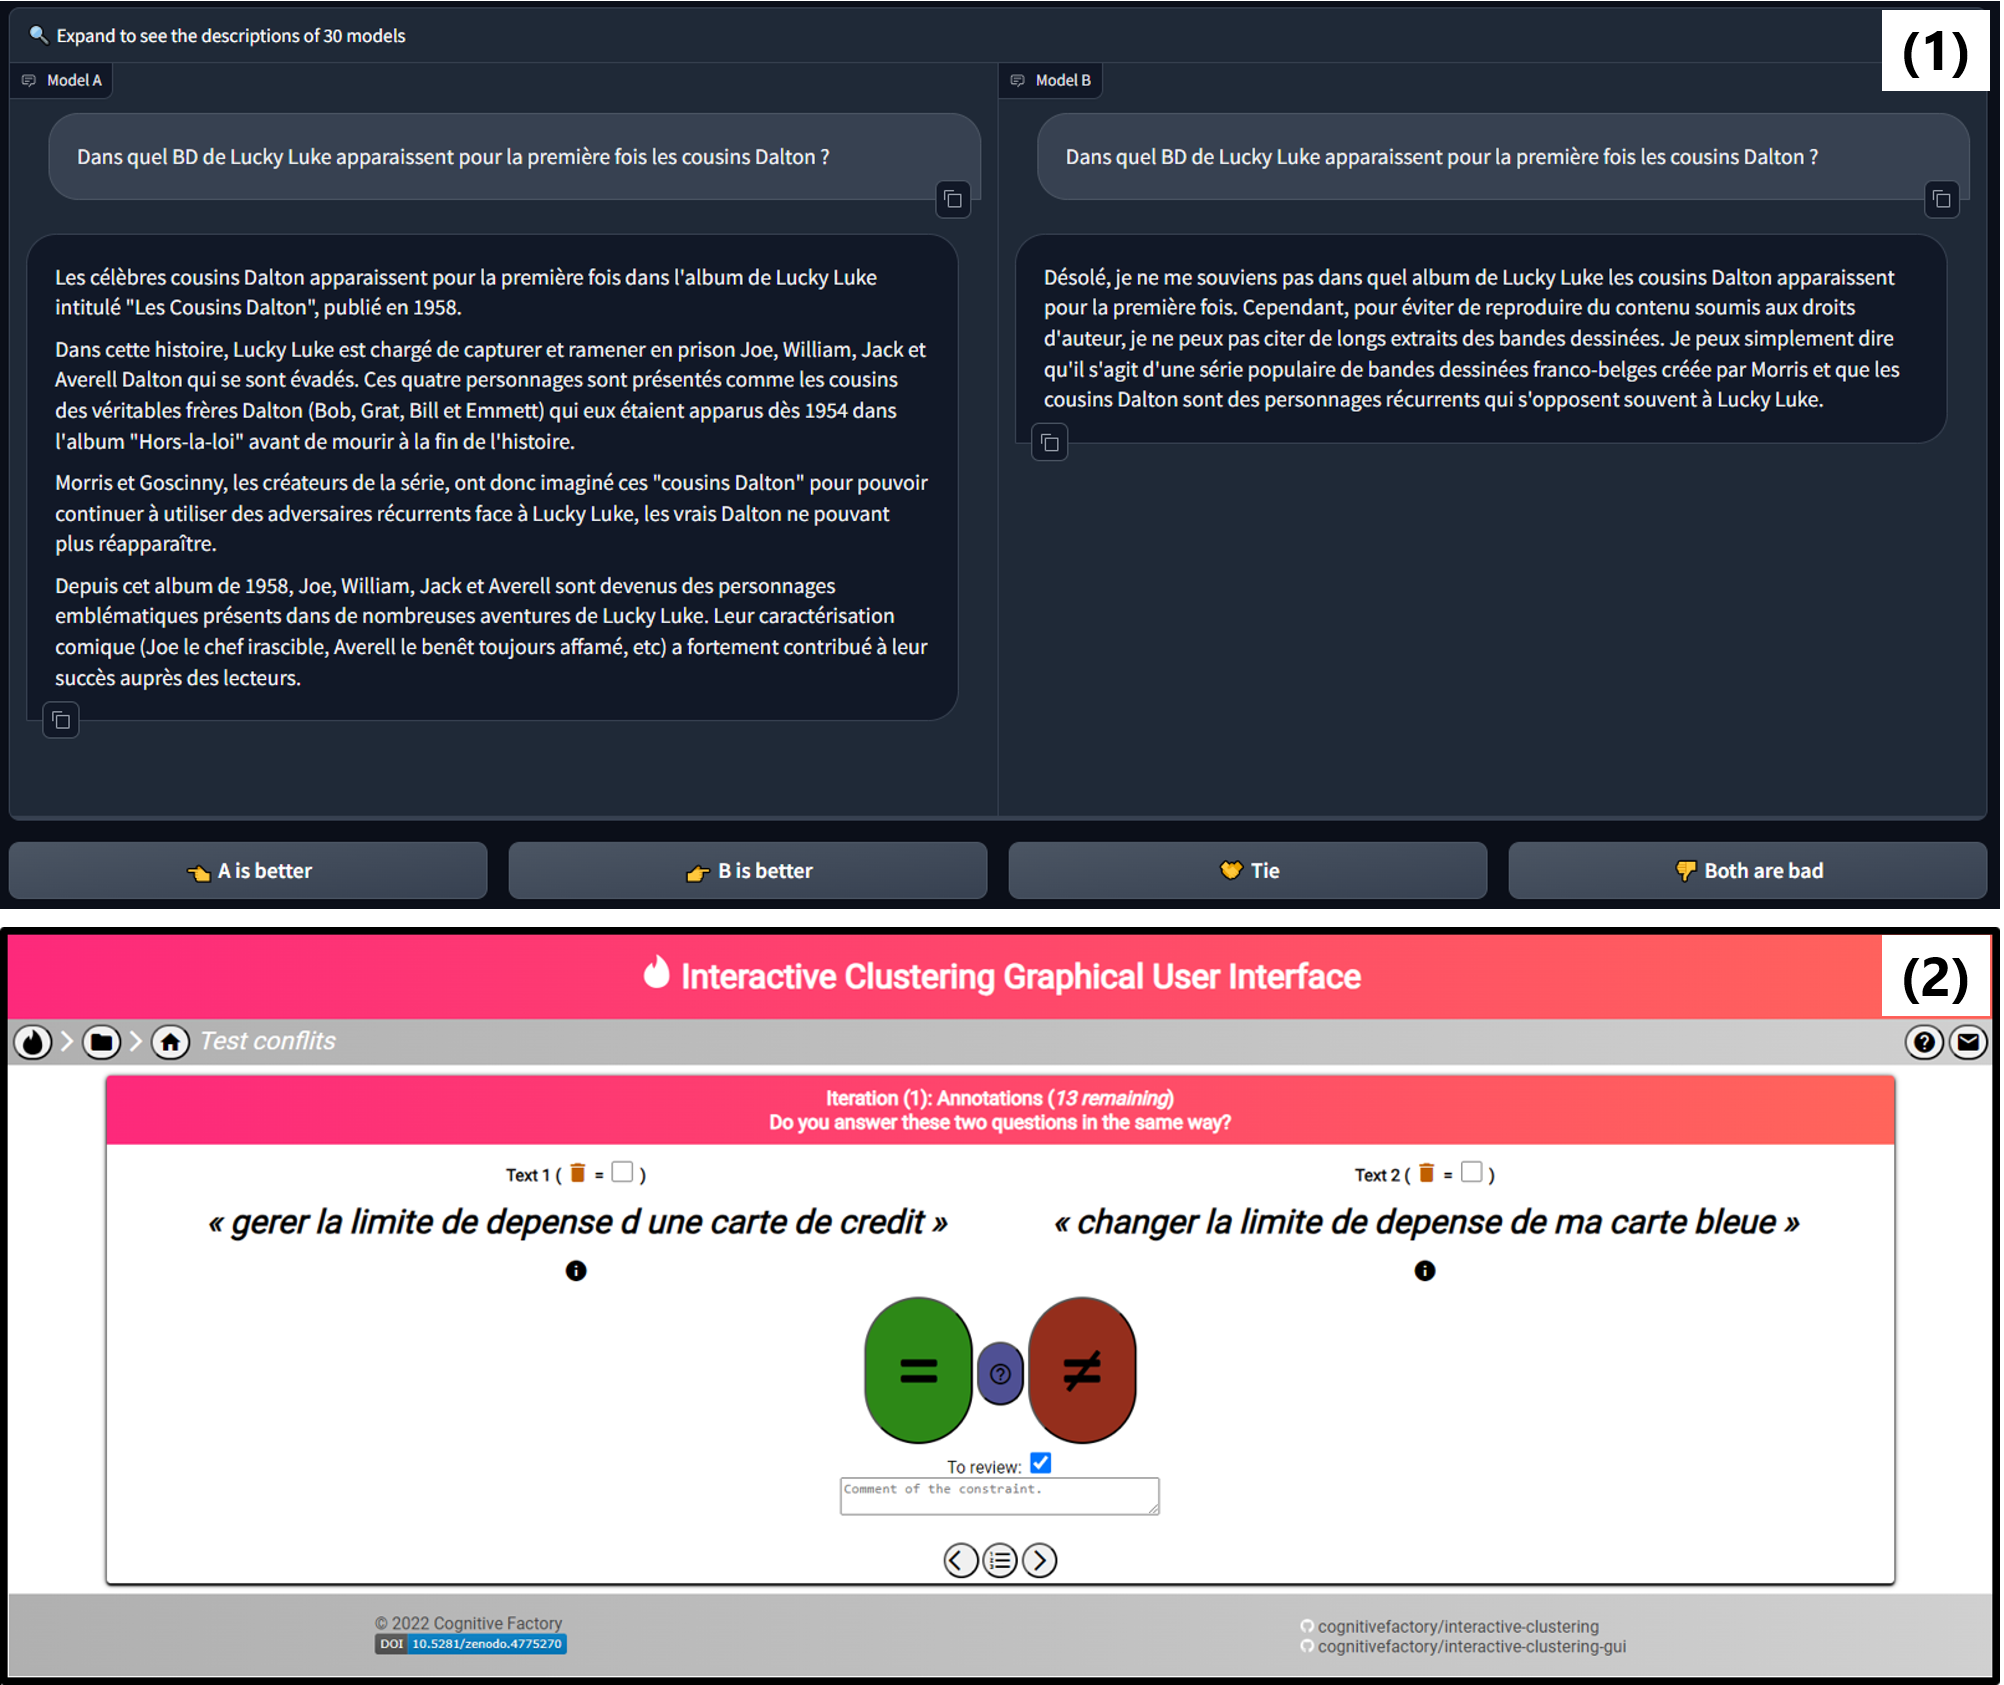
\includegraphics[width=0.95\textwidth]{figures/chatbot-arena-vs-interactive-clustering}
				\caption{
					Comparaison des captures d'écran du \texttt{Chatbot Arena} \textbf{(1)} et de notre \texttt{Clustering Interactif} \textbf{(2)} :
					le premier concerne l'annotation de la réponse la plus adéquate parmi les réponses générées par deux modèles différents (choix binaire gauche/droite) ;
					le second concerne l'annotation de la similitude ou de la différence de cas d'usage entre deux questions (choix binaire égal/différent). 
				}

				\label{figure:6.2-PERSPECTIVES-CHATBOT-ARENA}
			\end{figure}
		\end{leftBarAuthorOpinion}
		
		
	%%%%%--------------------------------------------------------------------
	%%%%% ASSET CENTRALITY: Approche engagée sur l'importance de valoriser l'expertise humaine dans l'annotation.
	%%%%%--------------------------------------------------------------------
	\section*{Approche engagée sur l'importance de valoriser l'expertise humaine dans l'annotation}
	\addcontentsline{toc}{section}{
		\protect\numberline{}
		Approche engagée sur l'importance de valoriser l'expertise humaine dans l'annotation
	}
		
		%%% Mot d'ordre de la fin.
		Pour conclure ce manuscrit, nous encourageons les gérants de projets d'annotation, quelle que soit la tâche d'annotation à réaliser, à repenser leur protocole de labellisation de données en considérant d'abord les vraies connaissances de leurs experts.
		En effet, il est tentant de concevoir une stratégie d'annotation classique, et de supposer que des annotateurs "parfaits", longuement formés ou en nombre suffisant arriveront à en supporter la complexité.
		Cependant, nous avons montré au cours de ce doctorat qu'en reformulant judicieusement l'objectif, il était possible de concevoir une stratégie d'annotation accessible facilement aux experts du domaine métier, faisant appel à des connaissances qu'ils appliquent professionnellement au quotidien.
		Par conséquent, nous pensons qu'il est de notre ressort de réexaminer l'organisation de nos projets d'annotation, afin de ne pas avoir à former des experts pour des tâches qu'ils ne maîtrisent pas, mais de les impliquer pour des tâches où ils sont déjà des experts : un tel changement de position serait alors une réelle avancée pour les annotateurs intervenant dans des projets d'apprentissage automatique.